\chapter{Fluid Flows \& Harmonic Functions}

\begin{proposition}
    Suppose $D \subseteq \mathbb{C} (= \mathbb{R}^2)$ and the following kind of flow fluid flowing through $D$.
    \begin{figure}[H]
        \centering
        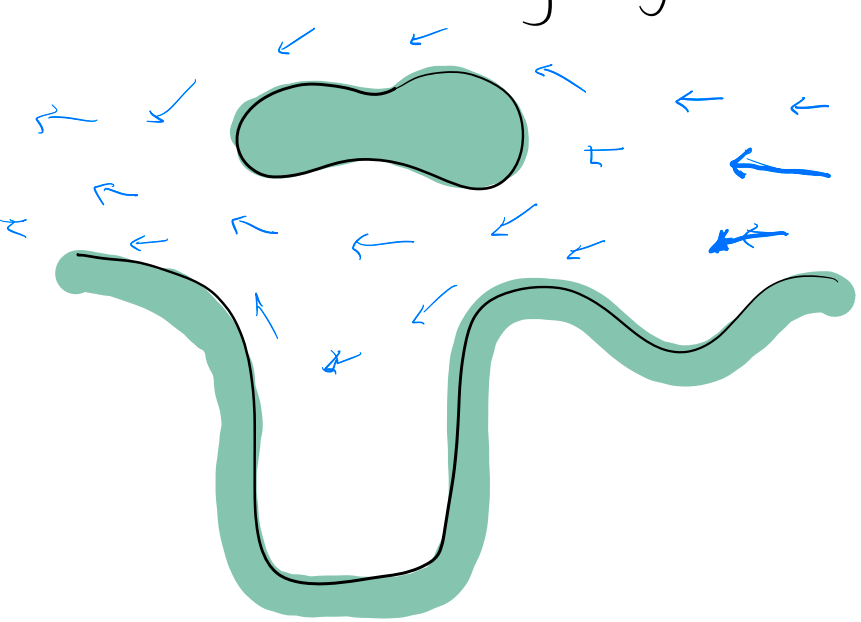
\includegraphics[width=0.5\textwidth]{LECTURE_19/graph.png}
        \caption{Fluid Flow through $D$}
    \end{figure}
    \textbf{We assume:}
    \begin{enumerate}
        \item[(i)] The flow is in a \textbf{steady state} (velocity doesn't change with time).
        \item[] The direction of the flow at $(x,y) \in D$ is given by a vector field $\mathbf{v}(x,y) = (u(x,y), v(x,y))$.
        \item[(ii)] the flow is \textbf{irrotational}, imagine a small paddle wheel at $(x,y)$, it doesn't rotate.
        \item[] \begin{figure}[H]
                  \centering
                  \begin{subfigure}{0.4\textwidth}
                      \centering
                      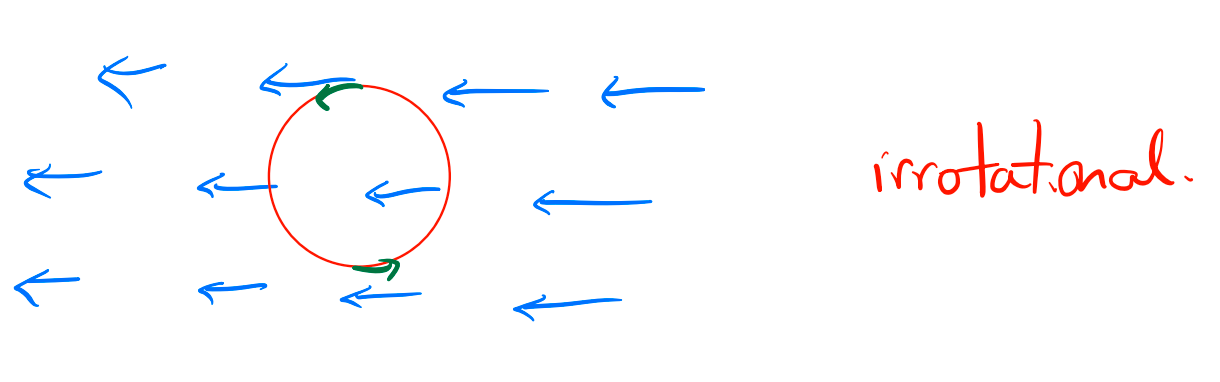
\includegraphics[width=\textwidth]{LECTURE_19/irrotational.png}
                      \caption{Irrotational Flow}
                  \end{subfigure}
                  \hfill
                  \begin{subfigure}{0.4\textwidth}
                      \centering
                      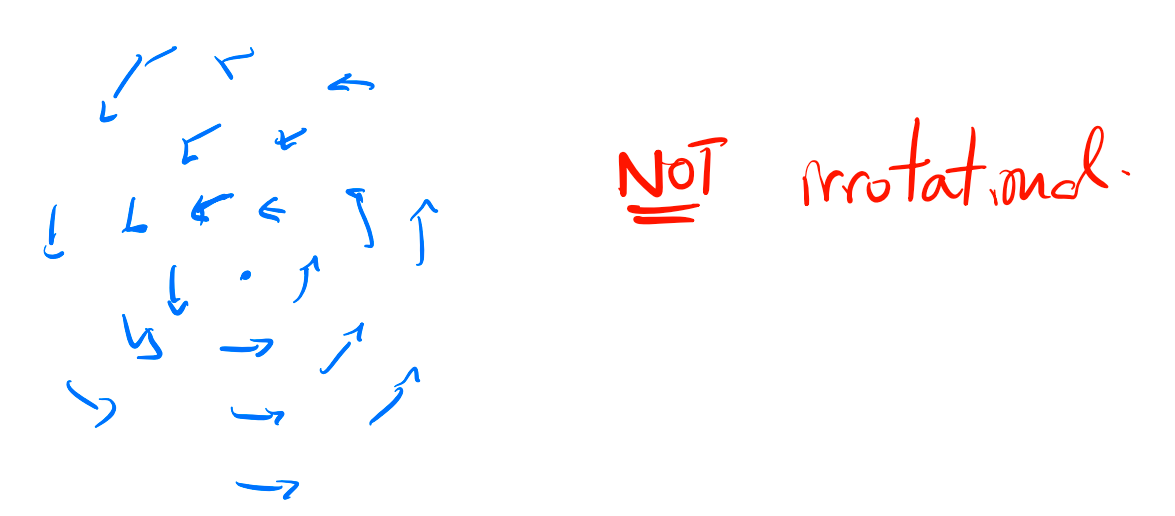
\includegraphics[width=\textwidth]{LECTURE_19/rotational.png}
                      \caption{Rotational Flow}
                  \end{subfigure}
              \end{figure}
        \item[] \textbf{Mathematically:} $\frac{\partial v}{\partial x} = \frac{\partial u}{\partial y}, \quad \forall (x,y) \in D$.
        \item[] You can think of $\frac{\partial v}{\partial x}$ as the change in vertical velocity as you move in the horizontal direction. Essentially, the amount of $x$ rotation (counter clockwise). Similarly, $\frac{\partial u}{\partial y}$ is the amount of $y$ rotation (clockwise). Therefore, if there is a horizontal rotation, there must be a vertical rotation to maintain irrotationality.
        \item[(iii)] The flow is \textbf{sourceless/sinkless}, no fluid is created or destroyed (incompressible).
        \item[] \textbf{Mathematically:} $\frac{\partial u}{\partial x} + \frac{\partial v}{\partial y} = 0, \quad \forall (x,y) \in D$.
        \item[] You can think of $\frac{\partial u}{\partial x}$ as the change in horizontal velocity as you move in the horizontal direction. Essentially, the amount of $x$ stretch/compression. Similarly, $\frac{\partial v}{\partial y}$ is the amount of $y$ stretch/compression. Therefore, if there is a horizontal stretch, there must be a vertical stretch to maintain the same volume.
    \end{enumerate}
\end{proposition}

\begin{remark}
    For a function $f(z)$ that is analytic in $D$, and the independent variable $z = x + iy$ where $x,y \in \mathbb{R}$, we can define $\frac{\partial}{\partial z}$ and $\frac{\partial}{\partial \overline{z}}$ as follows:
    \begin{align*}
        \frac{\partial}{\partial z} = \frac{1}2\left(\frac{\partial}{\partial x} - i\frac{\partial}{\partial y}\right), \quad \frac{\partial}{\partial \overline{z}} = \frac{1}2\left(\frac{\partial}{\partial x} + i\frac{\partial}{\partial y}\right)
    \end{align*}
\end{remark}

\begin{corollary}
    [Cauchy-Riemann Equations for Flows]
    If $\mathbf{v}(x,y) = (u(x,y), v(x,y))$ is a sourcelss irrotational flow then:
    \begin{enumerate}
        \item[(i)] $\Delta u = \frac{\partial^2 u}{\partial x^2} + \frac{\partial^2 u}{\partial y^2} = 0$.
        \item[(ii)] $\Delta v = \frac{\partial^2 v}{\partial x^2} + \frac{\partial^2 v}{\partial y^2} = 0$.
        \item[(iii)] $\overline{f} = u - iv$ is analytic in $D$ by the Cauchy-Riemann equations.
    \end{enumerate}

    \textbf{Furthermore,} there exists an analytic function $G$ on $D$ such that $G' = \overline{f}$ on $D$.
    \begin{proof}
        Why must there exist such a $G$?\\
        Because sources and irrotational flows imply $\int_\gamma \overline{f} dz = 0 \quad \forall$ closed curves $\gamma$ and vice-versa.
    \end{proof}
    Now then, by (the proof of) Morera's Theorem
    \begin{align*}
        G                 & = \phi + i \psi                                                                                                                                                                                \\
        \frac{dG}{dz}     & = \frac{1}2\left[\frac{\partial G}{\partial x} - i\frac{\partial G}{\partial y}\right]                                                                                                         \\
                          & = \frac{1}2\left[\left(\frac{\partial \phi}{\partial x} + i\frac{\partial \psi}{\partial x}\right) - i\left(\frac{\partial \phi}{\partial y} + i\frac{\partial \psi}{\partial y}\right)\right] \\
                          & \rightarrow \text{Now we can separate the real and imaginary parts}                                                                                                                            \\
                          & = \frac{1}2\left[\left(\frac{\partial \phi}{\partial x} + \frac{\partial \psi}{\partial y}\right) + i\left(\frac{\partial \psi}{\partial x} - \frac{\partial \phi}{\partial y}\right)\right]   \\
                          & \rightarrow \text{We know } \overline{f} = G' \text{ is analytic}                                                                                                                              \\
                          & \rightarrow \text{Then } G \text{ must be analytic and follow the Cauchy-Riemann equations}                                                                                                    \\
                          & \rightarrow \frac{\partial \phi}{\partial x} + \frac{\partial \psi}{\partial y} = 2\frac{\partial \phi}{\partial x}                                                                            \\
                          & \rightarrow \frac{\partial \psi}{\partial x} - \frac{\partial \phi}{\partial y} = 2\frac{\partial \psi}{\partial x}                                                                            \\
        G'= \overline{f}  & = \underbrace{\frac{\partial \phi}{\partial x}}_{u} + i\underbrace{\frac{\partial \psi}{\partial x}}_{-v}                                                                                      \\
        G' = \overline{f} & = \underbrace{\frac{\partial \psi}{\partial y}}_u - i\underbrace{\frac{\partial \phi}{\partial y}}_{v}
    \end{align*}
    So:
    \begin{align*}
        \nabla \phi & = (u,v) = \left(\frac{\partial \phi}{\partial x}, \frac{\partial \phi}{\partial y}\right)  \\
        \nabla \psi & = (-v,u) = \left(\frac{\partial \psi}{\partial x}, \frac{\partial \psi}{\partial y}\right)
    \end{align*}
    Thus:
    \begin{enumerate}
        \item[(i)] The level sets of $\{\phi = c\}$ are orthogonal to the flow
        \item[(ii)] The level sets of $\{\psi = c\}$ are flow lines.
    \end{enumerate}
    \textbf{$\phi$ is called the \underline{potential function}}
    \textbf{$\psi$ is called the \underline{stream function}.}
\end{corollary}

\begin{remark}
    \begin{itemize}
        \item[]
        \item The sets $\{\phi(x,y) = c\}$ are sets with equal potential energy at different $(x,y)$. Hence $\phi$ is called the potential function.
        \item The sets $\{\psi(x,y) = c\}$ are streamlines of the flow . Hence $\psi$ is called the stream function.
    \end{itemize}
\end{remark}

\begin{figure}[H]
    \centering
    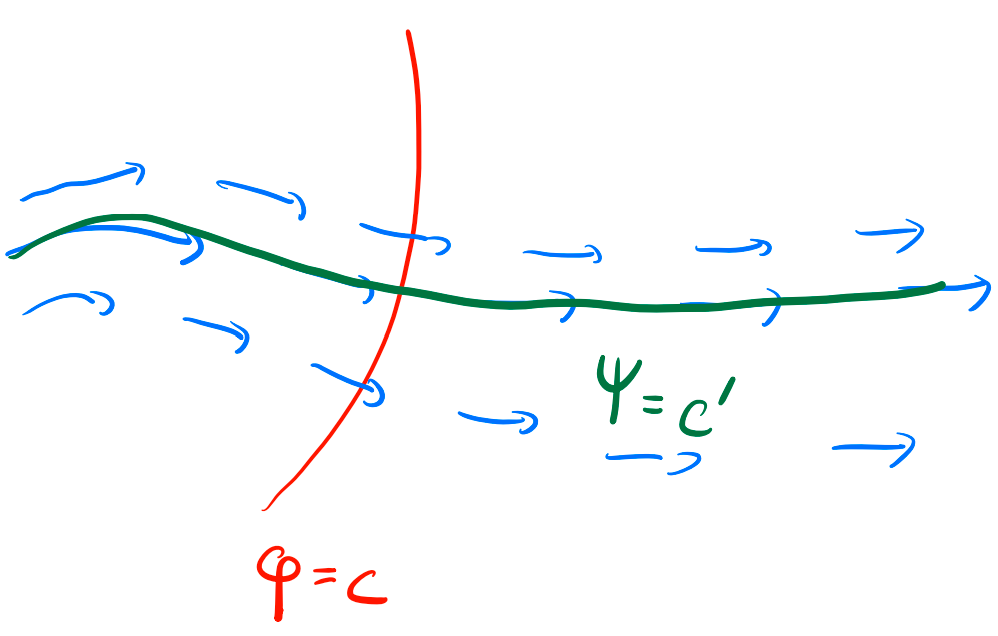
\includegraphics[width=0.5\textwidth]{LECTURE_19/potential-and-stream.png}
    \caption{Potential and Stream Functions}
\end{figure}

\begin{example}
    Find the flow lines of a sourceless irrotational flow past a wall of height $a$ (assuming take height is $>> a$).
    \begin{figure}[H]
        \centering
        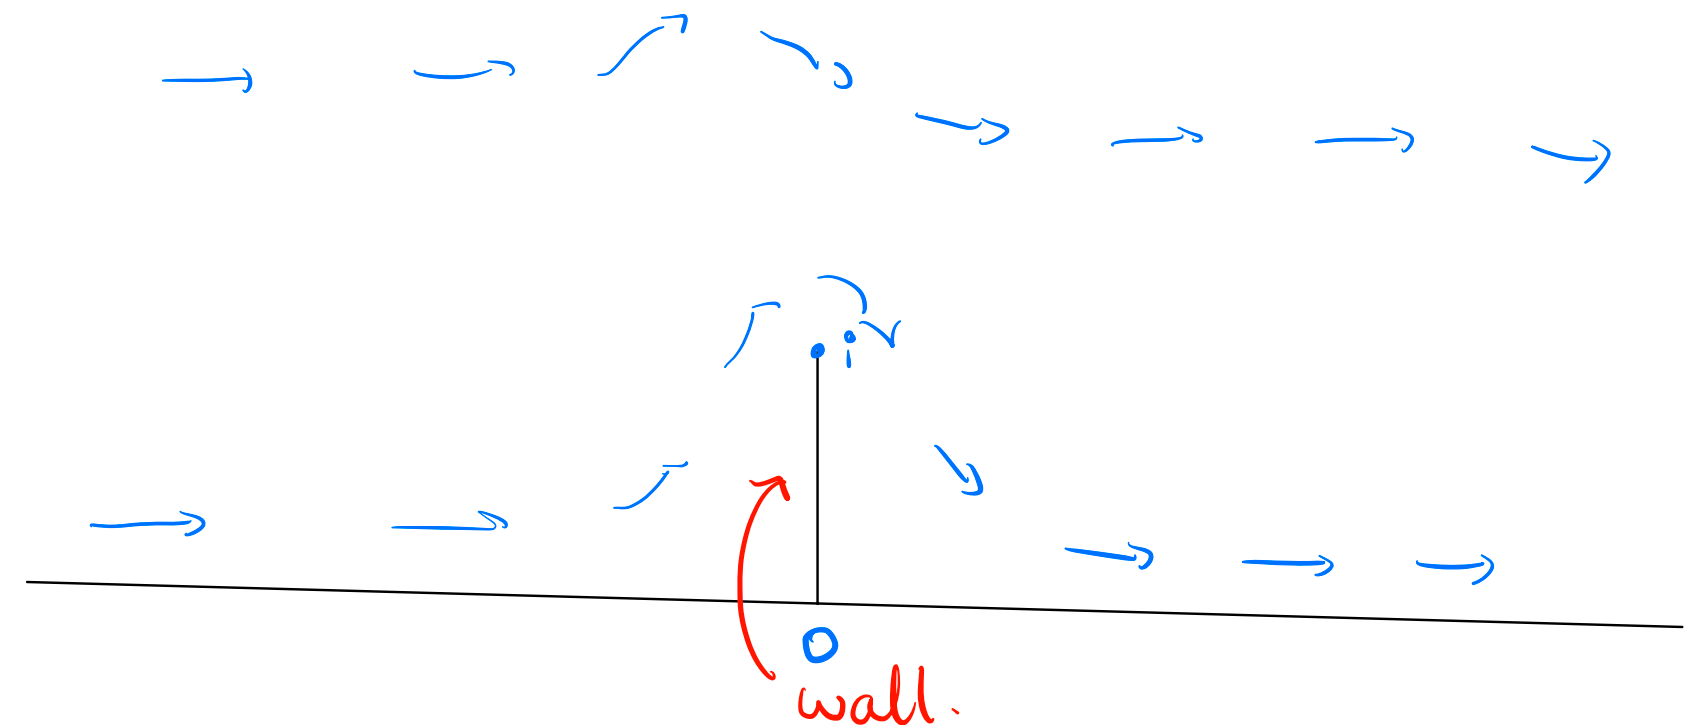
\includegraphics[width=0.5\textwidth]{LECTURE_19/graph1.png}
        \caption{Fluid Flow past a wall}
    \end{figure}
    \textbf{Solution:}
    Since the fluid can't flow through the wall, the flow lines must be orthogonal ($\nabla \phi = (u,v) = (0, v)$) to the wall on $x =0 ,\quad 0 \leq y \leq a$. We can solve this with conformal mapping. Our idea is we'll have a domain with a flow from left to right. We'll take the flow lines of that flow and map it to our domain with the wall. We'll then have the flow lines around the wall. \\
    Recall that $f(z) = a(z^2 - 1)^{1/2}$ defines a conformal map from $\mathbb{H}/\{it \in \mathbb{C} : 0 \leq t \leq a\}$ to the upper half plane, sending $f(-1) = f(1) = 0$. Let's consider the right moving flow in the pre-image $\mathbb{H}$:
    \begin{align*}
        (\tilde{u}, \tilde{v}) = (1, 0) \\
        \tilde{G} = z = x + iy
    \end{align*}
    Whose flow lines are given by $\{\Im(z) = y\}$ because there's only one component of velocity (there are no vertical flow lines), so we observe the flow at different values of $y$.\\
    The Image of these flow lines is under $f$ will be the flow lines around the wall $(a = 1)$.
    \begin{align*}
        f(x + iy) & = (z^2 - 1)^{\frac{1}2} = \sqrt{z -1}\sqrt{z + 1}                                                                                                                \\
                  & = \sqrt{(x + iy) - 1}\sqrt{(x + iy) + 1}                                                                                                                         \\
                  & = ((x -1) + y)^{1/2}((x+1) + y)^{1/2}                                                                                                                            \\
                  & = \pm|(x -1) + iy|^{1/2}e^{\frac{i}2\arg(x + iy - 1)}\times \pm|(x+1) + iy|^{1/2}e^{\frac{i}2\arg(x + iy + 1)}                                                   \\
                  & \rightarrow \arg(x + iy - 1) = \cos^{-1}\left(\frac{\Re(x + iy - 1)}{|x + iy - 1|}\right) = \cos^{-1}\left(\frac{x -1}{\sqrt{(x-1)^2 + y^2}}\right)              \\
                  & = ((x -1)^2 + y^2)^{1/4}e^{\frac{i}2\cos^{-1}(\frac{x -1}{\sqrt{(x-1)^2 + y^2}})}((x+1)^2 + y^2)^{1/4}e^{\frac{i}2\cos^{-1}(\frac{x + 1}{\sqrt{(x+1)^2 + y^2}})}
    \end{align*}
    \textbf{Note:} the root is multi-valued, because a conformal map is definite (and it doesn't make sense for a fluid to have two different directions in the same place), we have to choose a value. We choose the positive value to keep us in the upper-half plane.
    \begin{align*}
         & \text{x-component of the flow} =                                                                                                                                    \\
         & ((x- 1)^2 + y^2)^{1/4}((x+1)^2 + y^2)^{1/4}\cos(\frac{1}2\left(\cos^{-1}(\frac{x -1}{\sqrt{(x-1)^2 + y^2}}) + \cos^{-1}(\frac{x + 1}{\sqrt{(x+1)^2 + y^2})}\right)) \\
         & \text{y-component of the flow} =                                                                                                                                    \\
         & ((x- 1)^2 + y^2)^{1/4}((x+1)^2 + y^2)^{1/4}\sin(\frac{1}2\left(\cos^{-1}(\frac{x -1}{\sqrt{(x-1)^2 + y^2}}) + \cos^{-1}(\frac{x + 1}{\sqrt{(x+1)^2 + y^2})}\right))
    \end{align*}

    \begin{figure}[H]
        \centering
        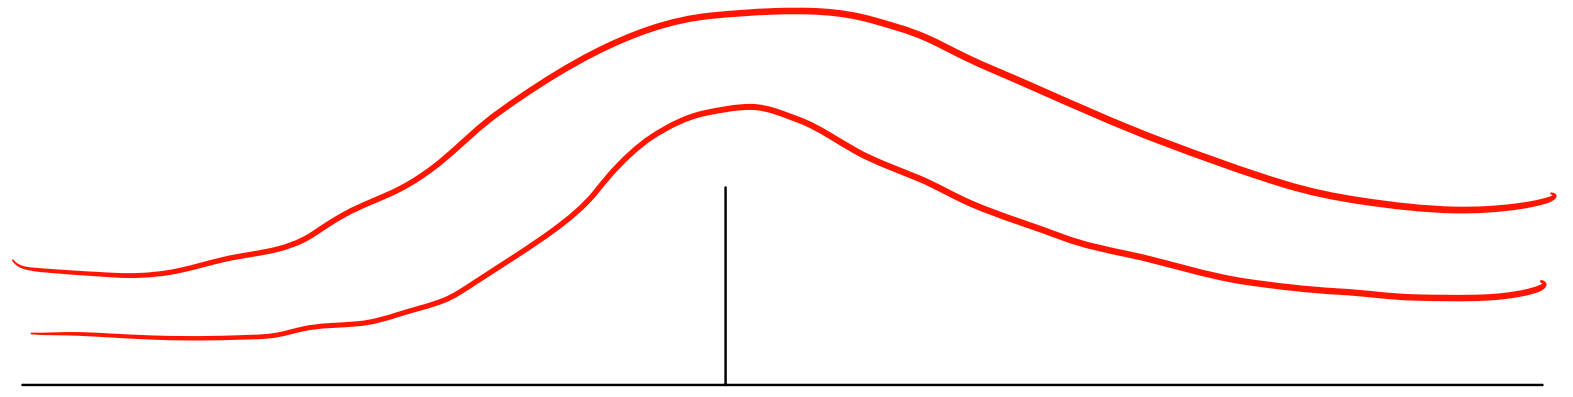
\includegraphics[width=0.5\textwidth]{LECTURE_19/resultant-flow.png}
        \caption{Flow Lines around the wall}

    \end{figure}

\end{example}

\begin{example}
    Find the flow lines of a sourceless irrotational flow past an infinitely deep trench.
    \begin{figure}[H]
        \centering
        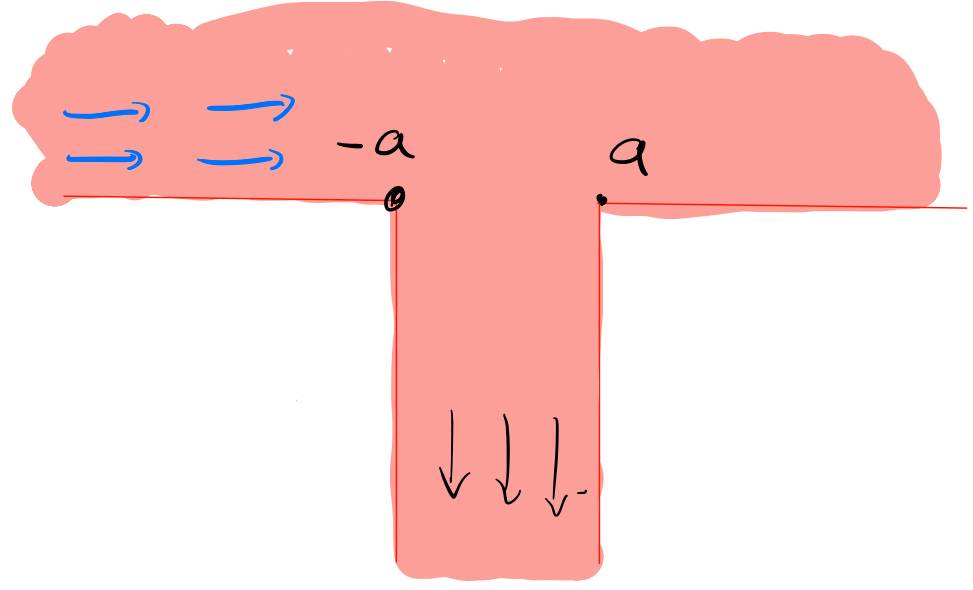
\includegraphics[width=0.5\textwidth]{LECTURE_19/trench.png}
        \caption{Fluid Flow past a trench}
    \end{figure}
    \textbf{Solution:}
    Recall that:
    \begin{align*}
        f(z) = \frac{2}\pi((z^2 -1)^{1/2} + \arcsin(\frac{1}z))
    \end{align*}
    Defines a conformal map from $\mathbb{H} \to$ the an infinitely deep trench from $-a$ to $a$.

    Consider the right moving flow
    \begin{align*}
        (\tilde{u}, \tilde{v}) = (1, 0)
    \end{align*}
    The flow lines through the trench are the image of the flow lines $\{\Im(z) = y\}$ under $f$.
    \begin{align*}
        f(x + iy) & = \sqrt{(x + iy) - 1}\sqrt{(x + iy) + 1}                                                                                                                                     \\
                  & = \frac{2}\pi[((x -1)^2 + y^2)^{1/4}e^{\frac{i}2\cos^{-1}(\frac{x -1}{\sqrt{(x-1)^2 + y^2}})}((x+1)^2 + y^2)^{1/4}e^{\frac{i}2\cos^{-1}(\frac{x + 1}{\sqrt{(x+1)^2 + y^2})}} \\
                  & + \arcsin(\frac{1}{x + iy})]
    \end{align*}

    \begin{figure}[H]
        \centering
        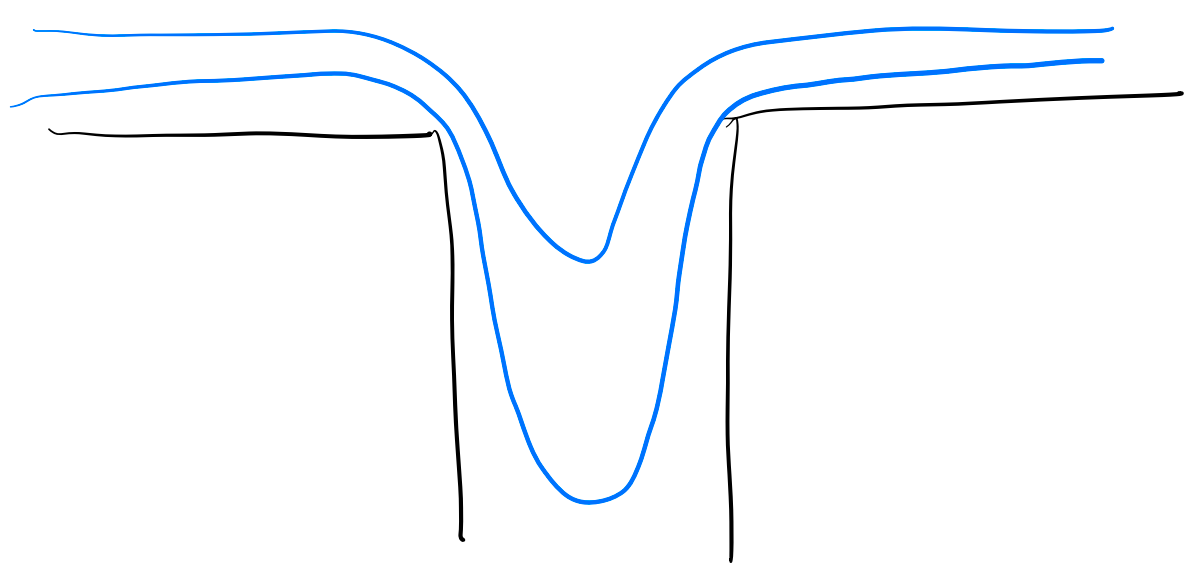
\includegraphics[width=0.5\textwidth]{LECTURE_19/trench-flow.png}
        \caption{Flow Lines through the trench}
    \end{figure}
\end{example}


\begin{example}
    [Fluid Flow Past a Solid Body]
    Lets Assume the flow is (locally) sourceless and irrotational.
    \begin{figure}[H]
        \centering
        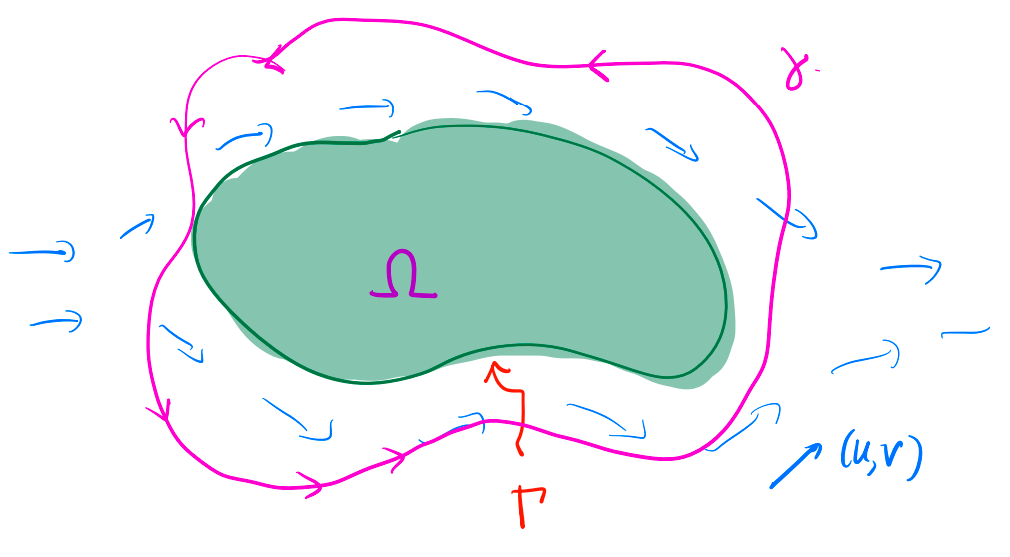
\includegraphics[width=0.75\textwidth]{LECTURE_19/flow-past-body.png}
        \caption{Fluid Flow past a solid body}
    \end{figure}
    \begin{itemize}
        \item $\Gamma$ is the simple closed curve, piecewise $C^1$ boundary around body.
        \item $\Omega$ is the region inside the body.
        \item $\gamma$ is some simple, closed, piecewise $C^1$, positively oriented curve such that $\Omega \subseteq$ inside$(\gamma)$.
        \item $\overline{f} = u - iv$ is analytic outside $\Omega$
    \end{itemize}
    We call $\tau = \frac{\gamma'}{|\gamma'|}$ the tangent unit vector to $\gamma$, $C$ the circulation of the flow around $\Omega$, and $ds = |\gamma'|dt$ the arc length element of $\gamma$.
    \begin{align*}
        C & = \int_\gamma f (\gamma') \cdot \tau \, ds                                                                               \\
          & = \int_\gamma (u + iv) \cdot \frac{\gamma'}{|\gamma'|} \, |\gamma'| \, dt                                                \\
          & = \int_\gamma \Re((u + iv) \cdot (\Re(\gamma') + i\Im(\gamma'))) \, dt \quad \text{Since the dot product is always real} \\
          & = \Re(\int_\gamma (u\Re(\gamma') - v\Im(\gamma')) \, dt)                                                                 \\
          & = \Re(\int_\gamma \overline{f} \gamma' \, dt)                                                                            \\
          & =\Re\left(\int_\gamma \overline{f} (\gamma')\gamma'dt\right) \quad \text{if } z = \gamma(t)                              \\
          & = \Re\left(\int_\gamma \overline{f} dz\right)                                                                            \\
    \end{align*}
    \textbf{Note:} $C$ does not depend on $\gamma$ by Cauchy's Theorem. Since $\overline{f}$ is analytic in $\Omega$.
    Since the flow goes around $\Omega$, and hence, there's no flow come out through the surface of the body:
    \begin{align*}
        (u,v) \cdot \vec{\eta} = 0 \quad \text{ on } \partial \Omega
    \end{align*}
    Where $\vec{\eta} = (\cos\theta, \sin\theta)$ (where $\theta = \arg(\vec{\eta})$) is the outward unit normal to $\partial \Omega$. So if you have a vertical wall, $\cos \theta = 0$ and thus $u\cos\theta = 0$ for all vertical flows, which makes sense since the flow is parallel to the wall. Similar for horizontal walls.\\
    So let's take the parametrization $\Gamma(t), \quad ds = |\Gamma'(t)|dt$ of $\partial \Omega$.
    \begin{align*}
        0 & = \int_{\partial \Omega =\Gamma} f(\Gamma(t)) \cdot \vec{\eta} \quad \Gamma'(t) \, dt
          & = \int_{\partial \Omega =\Gamma} (u + iv) \cdot (\cos\theta + i\sin\theta)
    \end{align*}
    \begin{align*}
        0 & = \int_{\partial \Omega =\Gamma} f \cdot \vec{\eta} \, dt                             \\
          & = \int_{\partial \Omega =\Gamma} (u + iv) \cdot (\cos\theta + i\sin\theta)
          & = \int_{\Gamma} \Re((u + iv) \cdot (-\tau_y + i\tau_x)) \, ds                         \\
          & = \int_{\Gamma} \Re((u + iv) \cdot (-\Im(\tau) + i\Re(\tau))) \, ds                   \\
          & = \int_{\Gamma} -u\Im(\tau) - v\Re(\tau) \, ds                                        \\
          & = \Im(\int_{\Gamma} \overline{f}(z) \, dz) = \Im(\int_{\Gamma} \overline{f}(z) \, dz)
    \end{align*}
    Assume the flow is uniform far from $\Omega$.
    \begin{figure}[H]
        \centering
        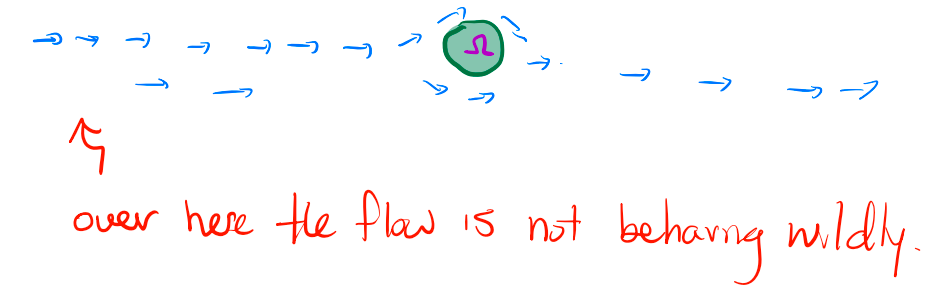
\includegraphics[width=\textwidth]{LECTURE_19/uniform.png}
        \caption{Uniform Flow}

    \end{figure}
    \begin{align*}
        \lim_{|z| \to \infty} \overline{f}(z) = a \in \mathbb{C}
    \end{align*}
    Thus, $\overline{f}$ has a removable singularity at $\infty$.
    i.e. If we set $w = \frac{1}z$ then $h(w) = \overline{f}(\frac{1}w)$ is analytic in $\{0 < |w| < \epsilon\}$ and bounded as $w \to 0$.\\
    Since $\overline{f}$ is analytic and has a removable singularity at $\infty$, it has a power series expansion at $\infty$.
    \begin{align*}
        \overline{f} = \sum_{k = 0}^{\infty}b_k(\frac{1}z)^k
    \end{align*}
    is valid for $|z|$ large.
    \begin{align*}
        \lim_{|z| \to \infty} \overline{f} & = \lim_{|z| \to \infty} \left(b_0 + \frac{b_1}z + \sum_{k = 2}^{\infty}b_k(\frac{1}z)^k\right) \\
        b_0                                & = a = \lim_{|z| \to \infty} f(z)                                                               \\
    \end{align*}
    Cauchy's Integral Formula can be used to find coefficients in a power series expansion.
    \begin{align*}
        b_k & = \frac{1}{2\pi i}\int_{|z| = R} \frac{\overline{f}(z)}{z^{k-1}} \, dz                         \\
            & = \frac{1}{2\pi i}\int_{|z| = R} \overline{f}(z) \, dz                                         \\
        b_1 & = \frac{C}{2\pi i} \quad \text{where} \quad C = \text{circulation of the flow around $\Omega$}
    \end{align*}
    This gives us the final result:
    \begin{align*}
        \overline{f}(z) = a + \frac{C}{2\pi i z} + \sum_{k = 2}^{\infty}b_k(\frac{1}z)^k
    \end{align*}

    \textbf{Our Goal: }To fix $C$, to get some $\overline{f}$ such that $\overline{f} \cdot \vec{\eta}|_\Gamma = 0$ on $\partial \Omega$.\\

\end{example}

\begin{proposition}
    [Kutta-Joukowski Theorem]
    Assume $\Omega$ has density $\rho$.\\
    \textbf{We can compute:} The total vertical force, $V$, and horizontal force $H$ on $\Omega$ due to the flow.
    \begin{align*}
        \boxed{V + iH = -\rho C a}
    \end{align*}
    If $a \in R$, then the only force is vertical, the lift force.
\end{proposition}

\begin{definition}
    [Unit Tangent \& Normal Vectors]
    Say we have some body $\Omega$ with boundary parametrized by $\Gamma(t)$. The unit tangent vector is:
    \begin{align}
        \tau = \frac{\Gamma'}{|\Gamma'|}
    \end{align}
    The unit normal vector is a clockwise $90^\circ$ rotation, which can be achieved by multiplying by $-i$, you can remember this by remembering how the vector $(1,0)$ rotates after multiplying by $i$ or $-i$.
    \begin{align}
        \eta = -i\tau = \frac{-i\Gamma'}{|\Gamma'|}
    \end{align}
    \begin{figure}[H]
        \centering
        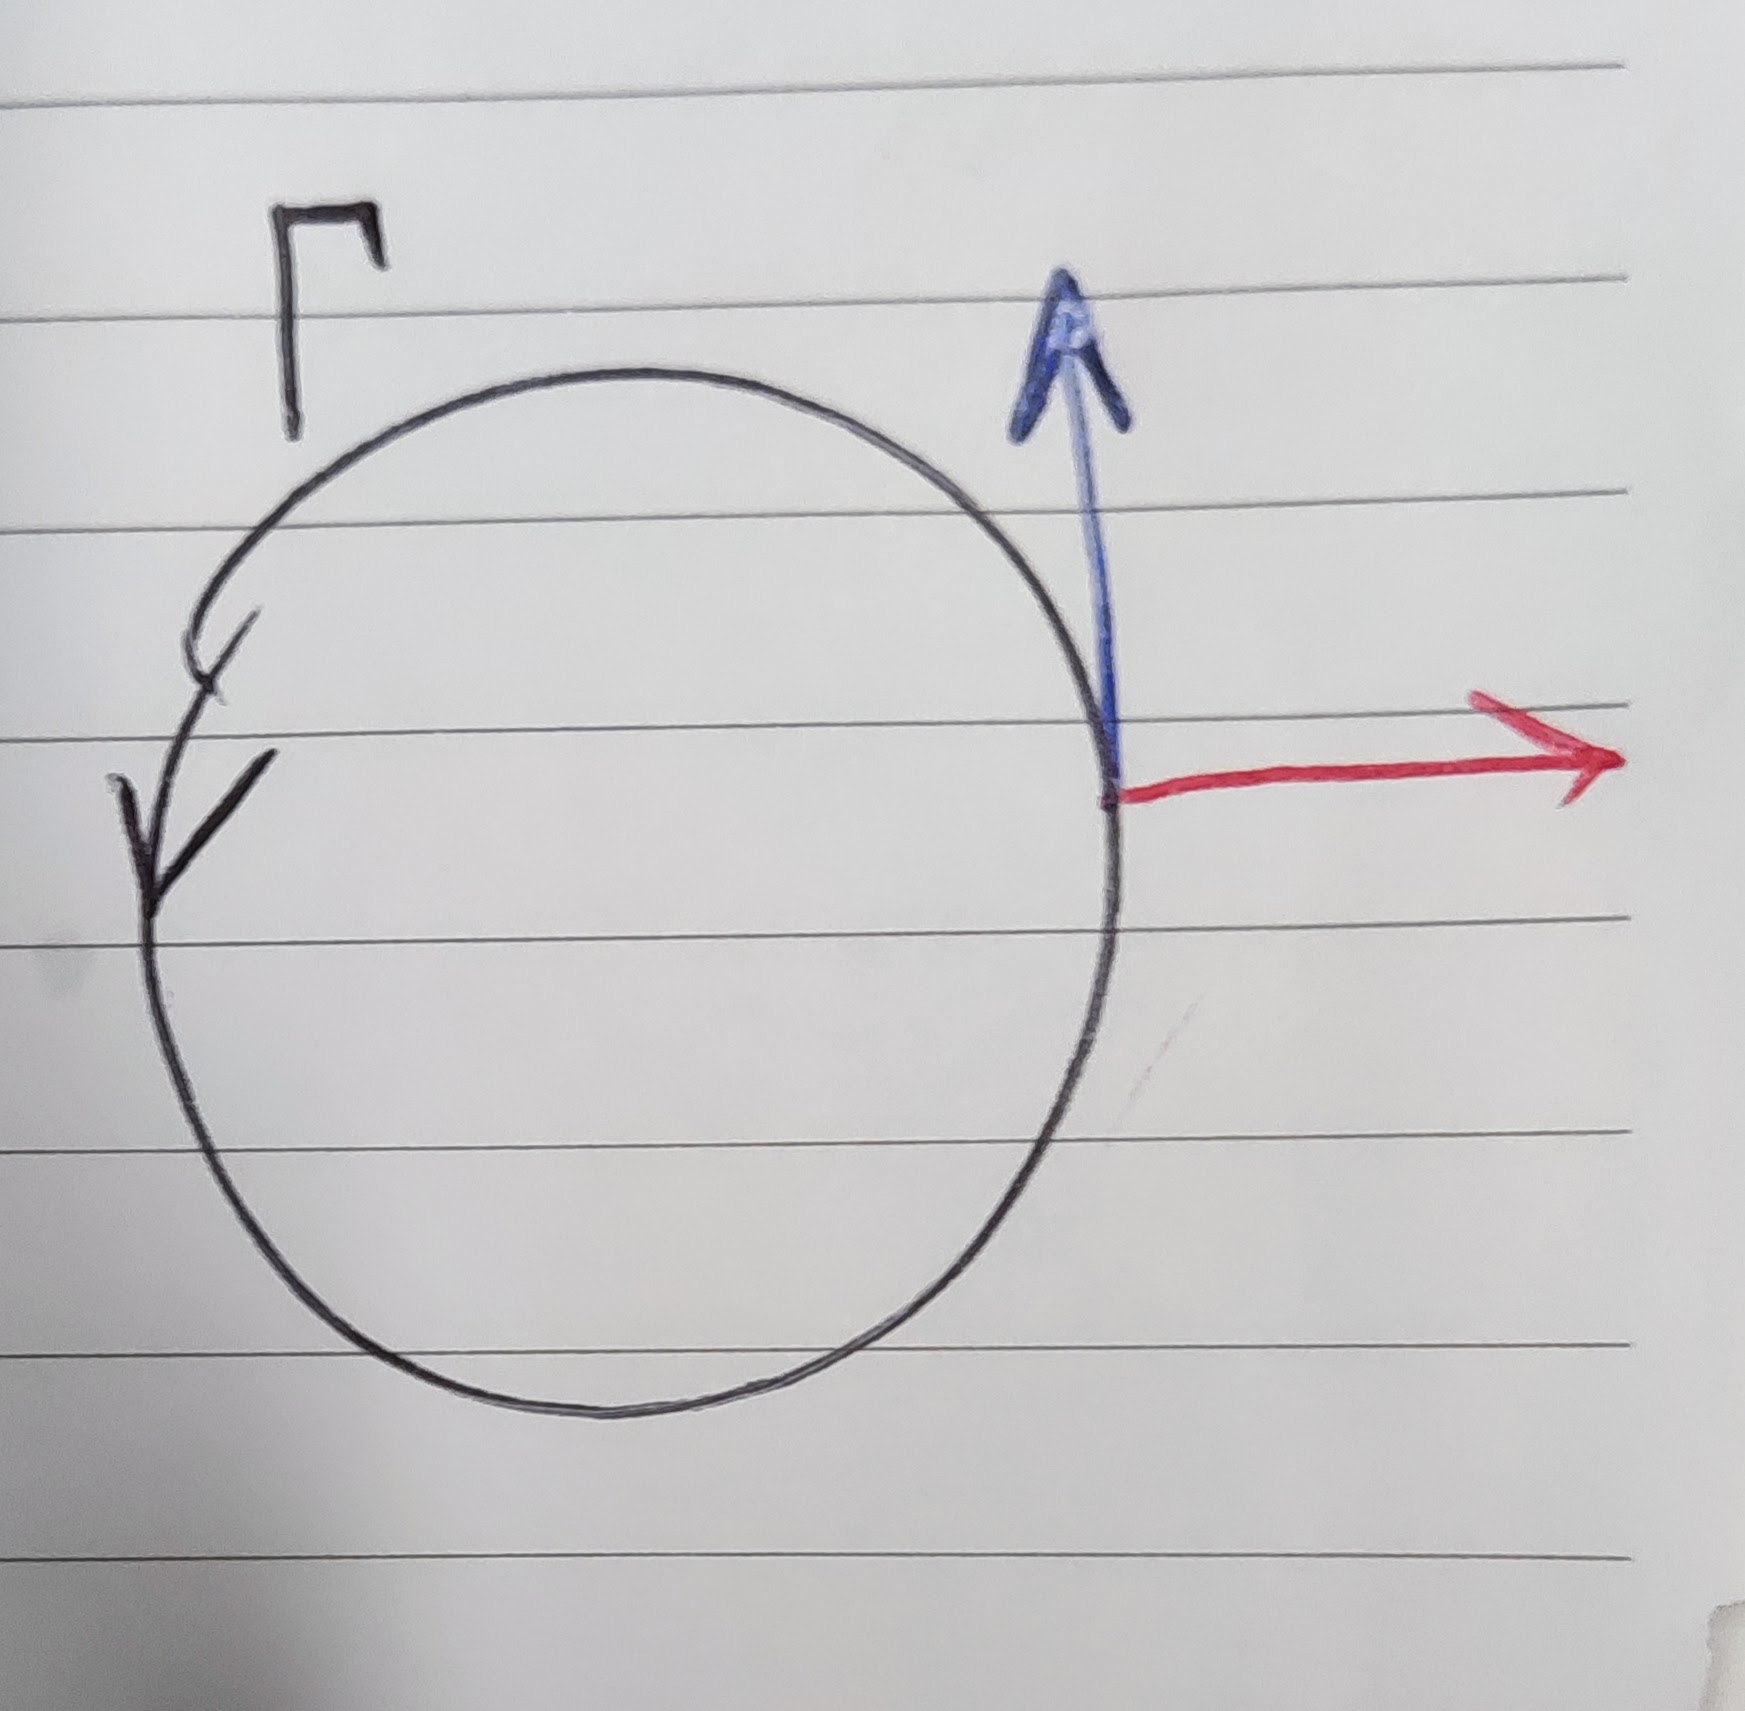
\includegraphics[width=0.5\textwidth]{LECTURE_19/unit.jpg}
        \caption{Unit Tangent and Normal Vectors}
    \end{figure}
\end{definition}

\begin{example}
    [Flow Past a Disk]
    \begin{align*}
        \Omega = \{|z| < 1\}                        \\
        \lim_{|z| \to \infty} \overline{f} = (1, 0) \\
    \end{align*}
    \begin{figure}[H]
        \centering
        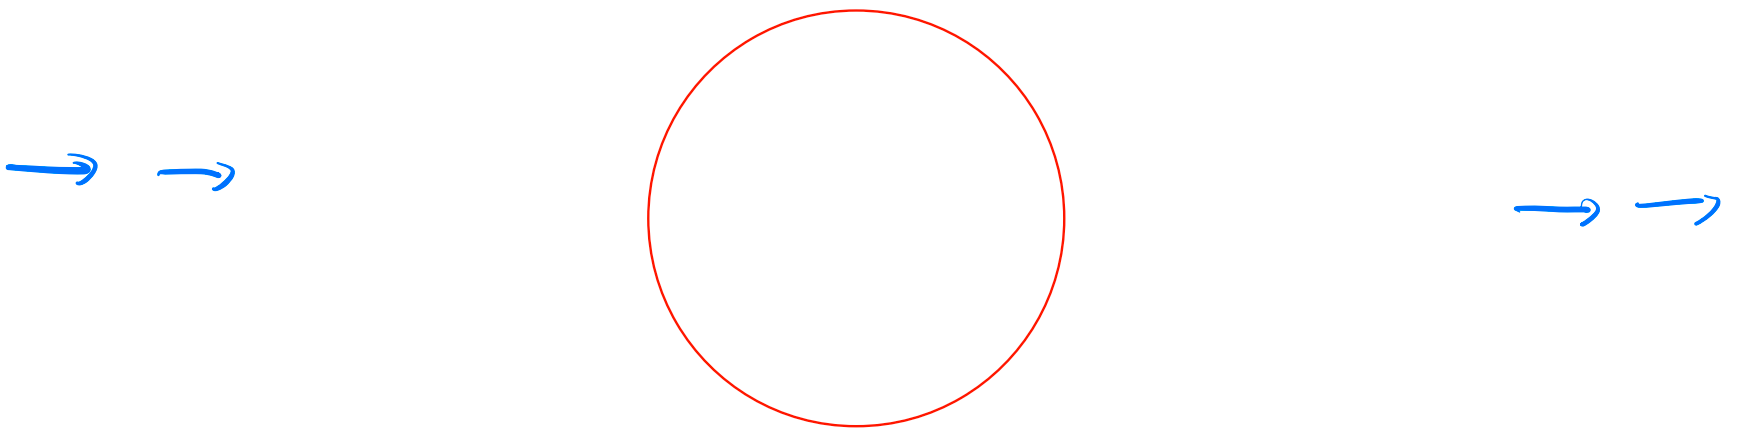
\includegraphics[width=\textwidth]{LECTURE_19/disk.png}
        \caption{Fluid Flow past a disk}
    \end{figure}
    \textbf{Therefore we want}
    \begin{align*}
        \overline{f} & = a + \frac{C}{2\pi i z} + \sum_{k = 2}^{\infty}b_k(\frac{1}z)^k \\
        \overline{f} & = 1 + \frac{C}{2\pi i z} + \sum_{k = 2}^{\infty}b_k(\frac{1}z)^k
    \end{align*}
    Such that on $\partial \Gamma$, $\Gamma(t) = e^{it}, \quad 0 \leq t \leq 2\pi$ which will parametrize a unit circle. First we find $\vec{\eta}$:
    \begin{align}
        \vec{\eta} & = -i\tau                       \\
                   & = -i\frac{\Gamma'}{|\Gamma'|}  \\
                   & = -i\frac{i e^{it}}{|ie^{it}|} \\
                   & = e^{it}
    \end{align}
    Now we want $\overline{f} \cdot \vec{\eta} = 0$ on $\partial \Omega$.
    \begin{align*}
        0 & = f(\Gamma) \cdot \eta                                            \\
          & = (u,v)\cdot(\cos\theta,\sin\theta)                               \\
          & = u\cos\theta + v\sin\theta                                       \\
          & = \Re((u - iv) (\cos\theta + i\sin\theta))                        \\
          & \rightarrow e^{i\theta} = \cos\theta + i\sin\theta                \\
          & = \Re((u - iv)e^{i\theta}) = \Re(\overline{f}(\Gamma)e^{i\theta})
    \end{align*}
    This way we can use what we know about $\overline{f}$
    \begin{align*}
        \Re\left[(1 + \frac{C}{2\pi i}e^{-i\theta} + \sum_{k = 2}^{\infty}b_k e^{-ik\theta})e^{i\theta}\right]       & = 0 \\
        \Re\left[\frac{C}{2\pi i} + e^{i\theta} + b_2e^{-i\theta} + \sum_{k = 3}^{\infty}b_k e^{i(1-k)\theta}\right] & = 0
    \end{align*}
    In order to make $\Re(\frac{C}{2\pi i}) = 0$, we must have $C$ be real so the whole term is imaginary.\\
    We can have $b_2e^{-i\theta}$ cancel out $e^{i\theta}$:
    \begin{align}
        \Re(e^{i\theta} + b_2e^{-i\theta}) & = \Re(\cos\theta + i\sin\theta + b_2(\cos(-\theta) + i\sin(-\theta))) \\
                                           & = \cos\theta + b_2\cos(-\theta)                                       \\
                                           & = \cos\theta + b_2\cos\theta = 0 \quad \text{if } b_2 = -1
    \end{align}
    Lastly, we can set $b_k = 0$ for $k \geq 3$ to make the sum term zero.\\
    In summary:
    \begin{align*}
        C\in \mathbb{R}, \quad b_2 = -1, \quad b_k = 0 \quad \forall k \geq 3
    \end{align*}
    Therefore:
    \begin{align*}
        \overline{f} = 1 - \frac{C}{2\pi i z} - \frac{1}{z^2}
    \end{align*}
    We can extend this analysis to other domains using conformal maps (e.g. conformal map $\phi$)\\ A common example is the Joukowski airfoil:
    \begin{align*}
        \Omega  & = {|z - z_0| < R}     \\
        \phi(z) & = (z + \frac{R^2}{z})
    \end{align*}

    \begin{figure}[H]
        \centering
        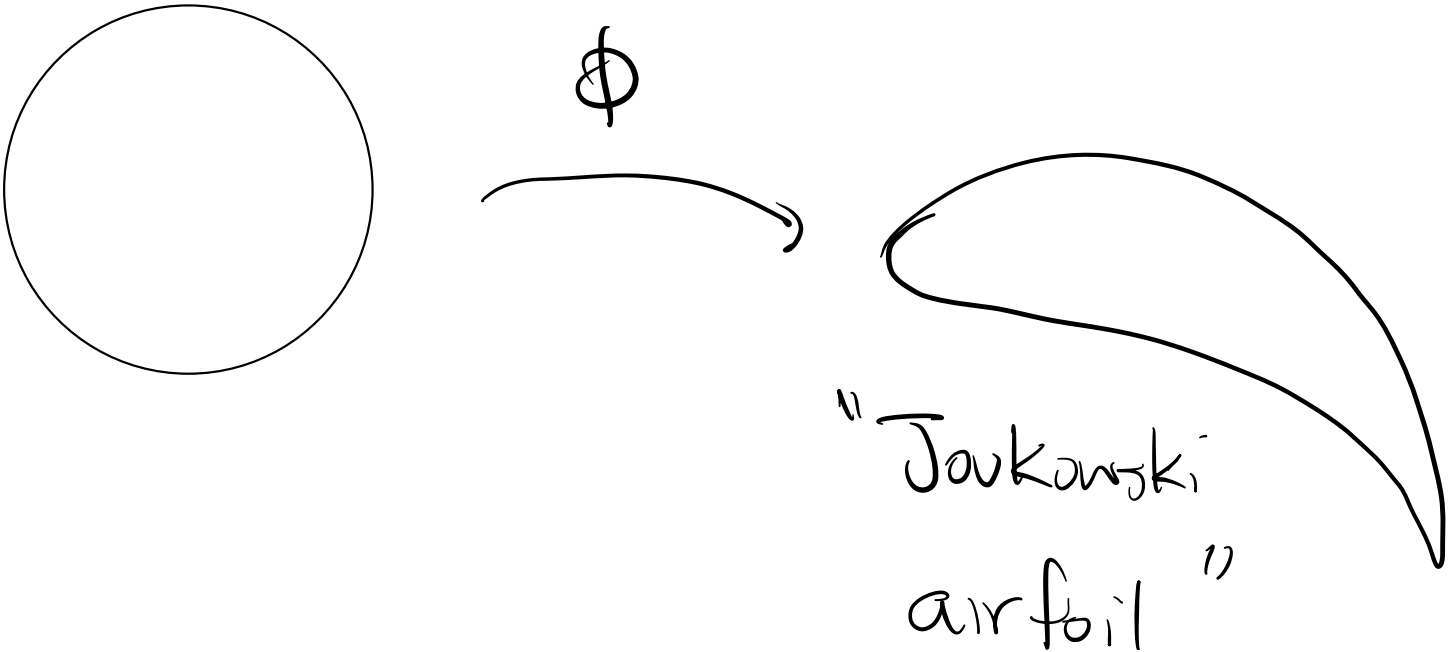
\includegraphics[width=0.5\textwidth]{LECTURE_19/airfoil.png}
        \caption{Conformal Map of a Disk}
    \end{figure}
    \begin{itemize}
        \item The circulation is determined by $z_0, \quad R$.
        \item The lift force is determined by $\Im(z_0)$.
    \end{itemize}
\end{example}
